\documentclass[a4paper,10pt]{article}
\usepackage[left=1in, right=1in, top=1in, bottom=1in]{geometry}
\usepackage{titlesec, xcolor, enumitem, hyperref, graphicx}
\usepackage{tikz}
\usepackage{fontawesome5}
\usepackage{fontspec}

% Define custom colors
\definecolor{darkblue}{RGB}{61,90,128}
\definecolor{lightblue}{RGB}{152,193,217}
\definecolor{graytext}{RGB}{100,100,100}

% Define custom font
\setmainfont{Arial}

% Title format
\titleformat{\section}{\large\bfseries\color{darkblue}}{}{0em}{}[\titlerule]

% Hyperlink setup
\hypersetup{
    colorlinks=true,
    linkcolor=darkblue,
    urlcolor=darkblue,
}

\begin{document}

\begin{minipage}{0.72\textwidth}
    {\LARGE\bfseries Sudipta Singha Rathi}\\[0.5em]
    {\large{Software Developer, Machine Learning Enthusiast, DevOps}}
\end{minipage}%
\hfill
\begin{minipage}{0.23\textwidth}
    \centering
    \begin{tikzpicture}
        \clip [rounded corners=0.5cm] (0,0) rectangle (3cm,3cm);
        \node at (1.5cm,1.5cm) {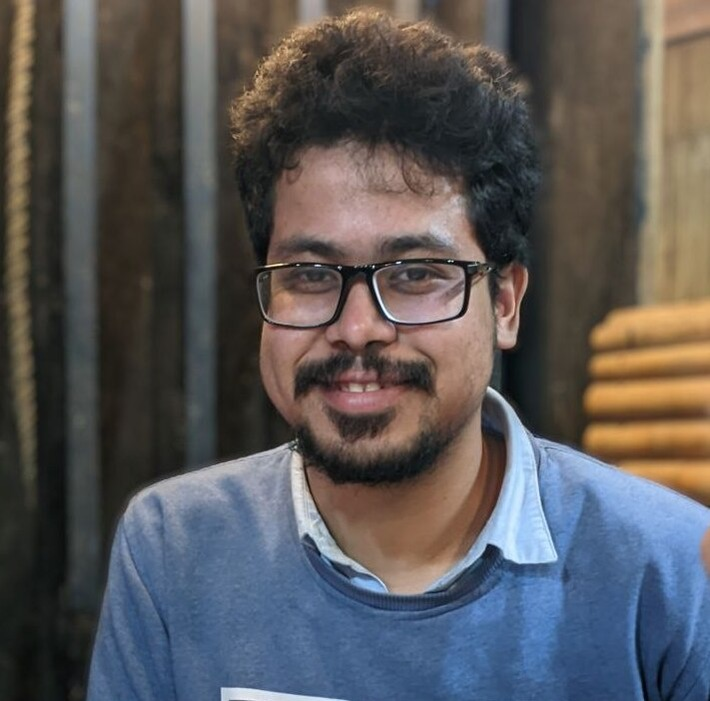
\includegraphics[width=3cm, height=3cm]{resources/profile.jpg}};
    \end{tikzpicture}
\end{minipage}

\section*{About Me}
I'm a 4th-year Computer Science and Engineering student at Jahangirnagar University. I love exploring new technologies and improving my skills.
Currently learning Machine Learning, Reinforcement Learning, Data Structures, System Design, Django, and DevOps.

\section*{Education}
\begin{itemize}[leftmargin=0.5cm]
    \item \textbf{Jahangirnagar University}\\
    BSc in Computer Science and Engineering
    \item \textbf{Milestone College}\\
    HSC in Science
    \item \textbf{Tetaigaon Rashid Uddin High School}\\
    SSC in Science
\end{itemize}

\section*{Skills}
\begin{itemize}[leftmargin=0.5cm]
    \item \textbf{Languages:} Java, C, C++, Python, LaTeX, Bash
    \item \textbf{Frameworks:} Django
    \item \textbf{Tools:} Linux, Git, WSL, Docker, AWS
    \item \textbf{Databases:} SQLite
\end{itemize}

\section*{Projects}
\begin{itemize}[leftmargin=0.5cm]
    \item \href{https://github.com/sudiptarathi2020/JUMCMS-Jahangirnagar-University-Medical-Center-Management-System.git}{JUMCMS}: A web application built with Django to improve medical center operations.
    \item \href{https://github.com/sudiptarathi2020/Software-Engineering-Lab-CSE404-Reports.git}{Software Engineering Lab Reports}: My software engineering lab reports.
    \item \href{https://github.com/sudiptarathi2020/Data-structures-and-Algorithms.git}{Data Structure and Algorithm Implementation}: Templates for data structures and algorithms.
    \item \href{https://github.com/sudiptarathi2020/Simple-Chess-Engine.git}{Chess Engine}: A simple chess engine using the minimax algorithm and alpha-beta pruning.
    \item \href{https://github.com/sudiptarathi2020/academic-report-maker.git}{Academic Report Maker}: A Django+React web application for generating academic reports.
    \item \href{https://github.com/sudiptarathi2020/puddle.git}{Puddle}: Created following a tutorial.
    \item \href{https://github.com/sudiptarathi2020/Problem-Solves.git}{Solved Problems on OJ}: Solutions to various problems on online judges.
    \item \href{https://github.com/sudiptarathi2020/problem-tutorials.git}{Lightoj Problem Tutorial Contributions}: My contributions to LightOJ problem tutorials.
\end{itemize}

\section*{Contact}
\begin{itemize}[leftmargin=0.5cm]
    \item \textbf{Address:} Jahangirnagar University, Savar, Dhaka
    \item \textbf{Phone:} +8801746-579065, +8801538-153490
    \item \textbf{Email:} \href{mailto:jucse29.408@gmail.com}{jucse29.408@gmail.com} | \href{mailto:rathisudipta99@gmail.com}{rathisudipta99@gmail.com} | \href{mailto:singha.stu2019@juniv.edu}{singha.stu2019@juniv.edu}
    \item \textbf{GitHub:} \href{https://github.com/sudiptarathi2020}{\faGithub \ sudiptarathi2020}
    % \item \textbf{LinkedIn:} \href{https://linkedin.com/in/your-profile}{\faLinkedin \ Your LinkedIn Profile}
\end{itemize}

\end{document}
